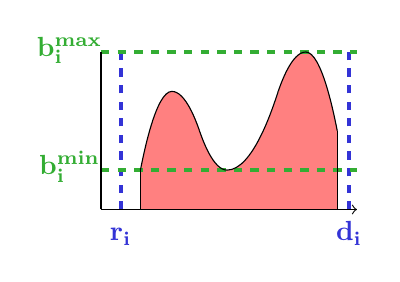
\begin{tikzpicture}
  [scale=0.5]
  \node (O) at (0,0) {};
  \fill[red!50] (1,0) -- (1,1) parabola bend (1.8,3)(2.51,2) -- (2.51,0);
  \fill[red!50] (2.49,0) -- (2.5,2) parabola bend (3.2,1) (4.511,3) -- (4.511,0) ;
  \fill[red!50] (4.489,0) -- (4.5,3) parabola bend (5.2,4) (6,2) -- (6,0);

  \node[label={[shift={(0,-0.7)}]\color{blue!80!black!80}$\mathbf{r_i}$}]  at (0.5,0) {};
  \node[label={[shift={(0,-0.7)}]\color{blue!80!black!80}$\mathbf{d_i}$}]  at (6.3,0) {};
  \draw[ultra thick,dashed,color=blue!80!black!80] (0.5,0) -- (0.5,4);
  \draw[ultra thick,dashed,color=blue!80!black!80] (6.3,0) -- (6.3,4);
  
    \node[label={[shift={(-0.4,-0.4)}]\color{green!60!black!80}$\mathbf{b_i^{min}}$}]  at (0,1) {};
    \node[label={[shift={(-0.4,-0.4)}]\color{green!60!black!80}$\mathbf{b_i^{max}}$}]  at (0,4) {};
    \draw[ultra thick,dashed,color=green!60!black!80] (0,1) -- (6.5,1);
    \draw[ultra thick,dashed,color=green!60!black!80] (0,4) -- (6.5,4);
  
  \draw (O.center) -- (0,4);
  \draw[->] (O.center) -- (6.5,0);
  
  \draw (1,1) -- (1,0);
  
  
  \draw (1,1) parabola bend (1.8,3)(2.5,2); 
  \draw (2.5,2) parabola bend (3.2,1) (4.5,3);
  \draw (4.5,3) parabola bend (5.2,4) (6,2);
  
  \draw (6,2) -- (6,0);
\end{tikzpicture}
